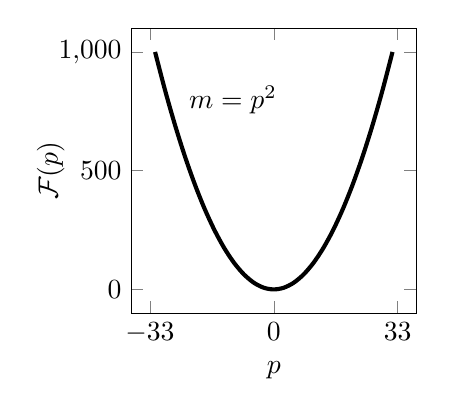
\begin{tikzpicture}
\begin{axis}
[scatter/classes={ a={mark=o,draw=blue}}, xlabel=$p$, ylabel=$ \mathcal{F}(p) $,
y label style={at={(axis description cs:-0.2,0.5)},anchor=south},
  height=5.2cm,
  width=5.2cm,
  xtick={-33,0,33}]
\addplot[smooth, line width=1.5pt, domain = -sqrt(1000):sqrt(1000), color=black] plot(\x,\x*\x) node[pos=0.1,inner sep=7pt, right] {$ m=p^2 $}; 
\end{axis}
	%\draw[->] (-3,0)--(3,0) node[right]{$x$};
	%\draw[->] (0,-2)--(0,4) node[left]{$y$};
	%\draw[smooth, line width=1.5pt, domain = -2:2, color=blue] plot(\x,\x*\x) node[right] {$ y=x^{2} $};
\end{tikzpicture}

